%\resizebox{\linewidth}{!}{%
\begin{tikzpicture}[
    declare function={unipdf(\x,\xl,\xu)= (\x>\xl)*(\x<\xu)*1/(\xu-\xl);}
]
	\begin{axis}[
	width=1.3\textwidth,
	xticklabels={,,},
	yticklabels={,,},
	ymin=0,
    	ymax=1.5,
	xlabel=\tiny{solutions $c$},
	ylabel=\tiny{$p_\beta(c | X)$},
	xticklabel style={inner sep=0pt},
	yticklabel style={inner sep=0pt}
	]
	\only<1>{\addplot[
	   red,
	   very thick,
	   domain=-2:2,
	   samples=201,
	]
	   { unipdf(x, -.35,.35) };}
	   
	%%
	\only<2>{\addplot[
	   red,
	   very thick,
	   domain=-2:2,
	   samples=201,
	]
	   {unipdf(x, -.5,.5) };}
	%%
	\only<3>{\addplot[
	   red,
	   very thick,
	   domain=-2:2,
	   samples=201,
	]
	   {unipdf(x, -1,1) };}
	\only<1->{%
	\draw[densely dashed] ({axis cs:0,0}|-{rel axis cs:0,0}) -- ({axis cs:0,0}|-{rel axis cs:0,1}) node[midway, above, sloped, yshift=-.1cm] {\tiny{optimal $c^\bot$}};}%
	  %%
	\only<4->{\addplot[
	   red,
	   very thick,
	   domain=-2:2,
	   samples=201,
	]
	   {unipdf(x, -1.5,1.5) };}
	\end{axis}
	\end{tikzpicture}%
%}